\documentclass{article}

% if you need to pass options to natbib, use, e.g.:
%     \PassOptionsToPackage{numbers, compress}{natbib}
% before loading neurips_2020

% ready for submission
% \usepackage{neurips_2020}

% to compile a preprint version, e.g., for submission to arXiv, add add the
% [preprint] option:
    \usepackage[preprint]{neurips_2020}

% to compile a camera-ready version, add the [final] option, e.g.:
%     \usepackage[final]{neurips_2020}

% to avoid loading the natbib package, add option nonatbib:
    %  \usepackage[nonatbib]{neurips_2020}

% \usepackage[utf8]{inputenc} % allow utf-8 input
% \usepackage[T1]{fontenc}    % use 8-bit T1 fonts
\usepackage{hyperref}       % hyperlinks
\usepackage{url}            % simple URL typesetting
% \usepackage{booktabs}       % professional-quality tables
% \usepackage{amsfonts}       % blackboard math symbols
% \usepackage{nicefrac}       % compact symbols for 1/2, etc.
% \usepackage{microtype}      % microtypography
\usepackage{caption}
\usepackage{graphicx}

\linespread{1.25}

\title{DpicNet: A Transfer Learning Approach Towards Intel Multiclass Image Classification Dataset}

% The \author macro works with any number of authors. There are two commands
% used to separate the names and addresses of multiple authors: \And and \AND.
%
% Using \And between authors leaves it to LaTeX to determine where to break the
% lines. Using \AND forces a line break at that point. So, if LaTeX puts 3 of 4
% authors names on the first line, and the last on the second line, try using
% \AND instead of \And before the third author name.

\author{%
  Xiaotong Niu \\
  Department of Computer Science\\
  Boston University\\
  Boston, MA 02215 \\
  \texttt{silnuext@bu.edu} \\
  \And
  Phumin Walaipatchara \\
  Department of Computer Science\\
  Boston University\\
  Boston, MA 02215 \\
  \texttt{phuminw@bu.edu} \\
}

\begin{document}

\maketitle

\begin{abstract}
  Abstract here
\end{abstract}

% ==========================================================================

\section{Introduction}

\subsection{Transfer Learning}

\subsection{Xception}

\subsection{Dataset}

The dataset that we are targeting is located at \href{https://www.kaggle.com/puneet6060/intel-image-classification}{Intel Multi-class Image Classification} containing images of natural scenes around the world. Originally, this dataset was used to host a image classification challenge by Intel. There are 25,000 images of size 150 x 150 pixels within 6 categories: buildings, forest, glacier, mountain, sea, and street. They are splitted into roughly 14,000 images for training, 3,000 images for testing, and 7,000 images for prediction. Images will be preprocessed to match the input requirement of the Xception model.

% ==========================================================================

\section{Prior Works}

\section{Methodology and Structure}

We conducted experiments on various fully-connected network structures on top on the transferred convolutional network from Xception. Our settings includes changing number of nodes in the hidden layers, adding more hidden layers, and imposing regularization (L1, L2, etc.) to the hidden layers. In all settings, all hidden layers are incorporated with a bias term. The experiments yield different performance on image classification as measured by categorical corss-entropy loss and accuracy, which are presented under Section 4 Result.

\subsection{No Regularization}
We started by constructing the hidden layers of the fully-connected part without any regularization
\subsubsection{Structure 1}

In this structure, we designed the top parts of DpicNet to have 2 hidden layers with 512 and 128 nodes, respectively. All hidden layers are incorporated with a bias term, but no regulatization is applied to either the weight or the bias term.

\subsubsection{Structure 2}

In this structure, we increased the number of nodes of 2 hidden layers from Structure 1 to be 2048 and 1024 nodes, respectively. All hidden layers are incorporated with a bias term, but no regularization is applied to either the weight or the bias term.

\subsubsection{Structure 3}

In this structure, we decreased the number of nodes of 2 hidden layers from Structure 1 to be 256 and 32 nodes, respectively. All hidden layers are incorporated with a bias term, but no regularization is applied to either the weight or the bias term.

\subsubsection{Structure 4}

In this structure, we increased the number of nodes of 2 hidden layers from Structure 1 to be 8192 and 1024 nodes, respectively. All hidden layers are incorporated with a bias term, but no regularization is applied to either the weight or the bias term.

\subsubsection{Structure 5}

In this structure, we increased the number of nodes of 2 hidden layers from Structure 1 to be 16384 and 4096 nodes, respectively. All hidden layers are incorporated with a bias term, but no regularization is applied to either the weight or the bias term.

\subsection{With Regularization}

We are going to add different types of regularization to our network and examine the difference in performance. We choose Structure 4 as a base structure and the regularization techniques to be experimented are L1, L2, and L1 and L2. We tested applying L1 regularization to both hidden layers; however, the network exhibits very poor performance with less than 20\% accuracy. Therefore, this setting is not included in this section. We also tested applying L1 regularization to one layer and L2 regularization to another layer, but this setting exhibits mediocre performance with about 67\% accuracy. Therefore, this setting is not included in this section as well.

\subsubsection{Structure 6}

In this structure, there are two hidden layers with 8192 and 1024 nodes, same as Structure 4, and those layers are incorporated with a bias term. In addition, L2 regularization is applied to both layers

\subsection{Three hidden layers with no Regularization}

Adding more hidden layers increases the model parameters while enables more capability to fit the data better. We are going to experiment whether adding more layers (from 2 to 3) can decrease the loss and increase the accuracy on the data (training, testing, predict). Moreover, we are going to examine the tradeoff between growing parameters, which requires more training time and consumes more space, and accuracy on the data.

\subsubsection{Structure 7}

Based on Structure 4, this structure differs by adding one more hidden layer on top of the existing hidden layers in Structure 4 with 256 nodes. All hidden layers are incorporated with a bias term and no regularization of any kind is applied to any hidden layer.

\subsubsection{Structure 8}

This structure is almost identical with Structure 7, except that the number of nodes in the newly added hidden layer is changed to 512.

\subsection{}

% ==========================================================================

\section{Results}
We recorded the loss and accuracy of each structure on training and testing dataset. Loss function used is categorical cross-entropy loss function. The batch size for all experiments is 32. 

\subsection{Training Data}
Because of batch size of 32, each epoch contains 439 steps. The experiment result of each structure is shown in Table 1. From the experiment result, Structure 2, 4, and 7 are outstanding in terms of accuracy at epoch 10. Structure 6, which incorporated L2 regularization to both layers, does not exhibit impressive performance despite training up to 40 epochs. Structure 7 and 8, which have 3 hidden layers with different number of nodes in the last hidden layer, performs well compared to Structure 1 - 4; however, adding more hidden layer does not significantly improve the performance on the training dataset.

\begin{table}[]
  \centering
  \begin{minipage}[b]{0.23\linewidth}
  \tiny
  \begin{tabular}{|c|c|c|}
    \hline
    Epoch&Loss&Accuracy\\
    \hline
    1&0.7697&0.781\\
    \hline
    2&0.3522&0.8758\\
    \hline
    3&0.2424&0.9120\\
    \hline
    4&0.1798&0.9362\\
    \hline
    5&0.1248&0.9557\\
    \hline
    6&0.1135&0.9608\\
    \hline
    7&0.1253&0.9589\\
    \hline
    8&0.0786&0.9734\\
    \hline
    9&0.0696&0.9786\\
    \hline
    10&0.0713&0.9784\\
    \hline
  \end{tabular}
  \caption*{Structure 1}
  \end{minipage}
  \hspace{0.5cm}
  \begin{minipage}[b]{0.23\linewidth}
  \tiny
  \begin{tabular}{|c|c|c|}
    \hline
    Epoch&Loss&Accuracy\\
    \hline
    1&1.0170&0.7748\\
    \hline
    2&0.3853&0.8619\\
    \hline
    3&0.2634&0.9043\\
    \hline
    4&0.1818&0.9348\\
    \hline
    5&0.1483&0.9479\\
    \hline
    6&0.1179&0.9577\\
    \hline
    7&0.0871&0.9701\\
    \hline
    8&0.1059&0.9672\\
    \hline
    9&0.0648&0.9800\\
    \hline
    10&0.0526&0.9838\\
    \hline
  \end{tabular}
  \caption*{Structure 2}
  \end{minipage}
  \hspace{0.5cm}
  \begin{minipage}[b]{0.23\linewidth}
  \tiny
  \begin{tabular}{|c|c|c|}
    \hline
    Epoch&Loss&Accuracy\\
    \hline
    1&0.7723&0.7590\\
    \hline
    2&0.3895&0.8669\\
    \hline
    3&0.2822&0.9015\\
    \hline
    4&0.2205&0.9220\\
    \hline
    5&0.1826&0.9384\\
    \hline
    6&0.1295&0.9555\\
    \hline
    7&0.1031&0.9648\\
    \hline
    8&0.1051&0.9656\\
    \hline
    9&0.0784&0.9730\\
    \hline
    10&0.0912&0.9705\\
    \hline
  \end{tabular}
  \caption*{Structure 3}
  \end{minipage}
  \\
  \begin{minipage}[b]{0.23\linewidth}
  \tiny
  \begin{tabular}{|c|c|c|}
    \hline
    Epoch&Loss&Accuracy\\
    \hline
    1&1.7312&0.7761\\
    \hline
    2&0.3870&0.8603\\
    \hline
    3&0.2559&0.9063\\
    \hline
    4&0.1886&0.9333\\
    \hline
    5&0.1396&0.9513\\
    \hline
    6&0.1151&0.9618\\
    \hline
    7&0.0848&0.9726\\
    \hline
    8&0.0832&0.9734\\
    \hline
    9&0.0846&0.9748\\
    \hline
    10&0.0515&0.9840\\
    \hline
  \end{tabular}
  \caption*{Structure 4}
  \end{minipage}
  \hspace{0.5cm}
  \begin{minipage}[b]{0.23\linewidth}
  \tiny
  \begin{tabular}{|c|c|c|}
    \hline
    Epoch&Loss&Accuracy\\
    \hline
    1&2.4641&0.7775\\
    \hline
    2&0.3616&0.8706\\
    \hline
    3&0.2905&0.9042\\
    \hline
    4&0.2051&0.9287\\
    \hline
    5&0.1535&0.9471\\
    \hline
    6&0.1257&0.9583\\
    \hline
    7&0.1538&0.9603\\
    \hline
    8&0.0834&0.9722\\
    \hline
    9&0.0683&0.9776\\
    \hline
    10&0.0730&0.9797\\
    \hline
  \end{tabular}
  \caption*{Structure 5}
  \end{minipage}
  \hspace{0.5cm}
  \begin{minipage}[b]{0.23\linewidth}
  \tiny
  \begin{tabular}{|c|c|c|}
    \hline
    Epoch&Loss&Accuracy\\
    \hline
    1&11.6508&0.7146\\
    \hline
    2&2.7279&0.7545\\
    \hline
    3&2.0377&0.7770\\
    \hline
    4&2.0157&0.7779\\
    \hline
    5&1.7358&0.7926\\
    \hline
    6&1.5305&0.8003\\
    \hline
    7&1.3250&0.8088\\
    \hline
    8&1.2319&0.8123\\
    \hline
    9&1.1533&0.8154\\
    \hline
    10&1.0536&0.8180\\
    \hline
    20&0.7546&0.8336\\
    \hline
    30&0.6780&0.8423\\
    \hline
    40&0.6588&0.8439\\
    \hline
  \end{tabular}
  \caption*{Structure 6}
  \end{minipage}
  \\
  \begin{minipage}[b]{0.23\linewidth}
  \tiny
  \begin{tabular}{|c|c|c|}
    \hline
    Epoch&Loss&Accuracy\\
    \hline
    1&1.4817&0.7720\\
    \hline
    2&0.3707&0.8663\\
    \hline
    3&0.2519&0.9057\\
    \hline
    4&0.1884&0.9317\\
    \hline
    5&0.1469&0.9512\\
    \hline
    6&0.1170&0.9632\\
    \hline
    7&0.0929&0.9694\\
    \hline
    8&0.0954&0.9708\\
    \hline
    9&0.0886&0.9721\\
    \hline
    10&0.0597&0.9818\\
    \hline
  \end{tabular}
  \caption*{Structure 7}
  \end{minipage}
  \hspace{0.5cm}
  \begin{minipage}[b]{0.23\linewidth}
  \tiny
  \begin{tabular}{|c|c|c|}
    \hline
    Epoch&Loss&Accuracy\\
    \hline
    1&1.3941&0.7753\\
    \hline
    2&0.3921&0.8603\\
    \hline
    3&0.2674&0.9026\\
    \hline
    4&0.1950&0.9303\\
    \hline
    5&0.1589&0.9466\\
    \hline
    6&0.1189&0.9608\\
    \hline
    7&0.0974&0.9676\\
    \hline
    8&0.0669&0.9778\\
    \hline
    9&0.0771&0.9766\\
    \hline
    10&0.0724&0.9780\\
    \hline
  \end{tabular}
  \caption*{Structure 8}
  \end{minipage}
  \caption{Accuracy and Loss on Training Data}
  \label{t1:acc_loss_train_tab}
\end{table}

\subsection{Testing Data}

After training, each structure was tested on testing data using batch size of 32 and the testing was done after 94 steps. The performance is evaluated based on accuracy on the testing data and shown in Table 2. Structure 3 performs the best among all structures experimented despite no regularization applied and less hidden layers.

\begin{table}[]
    \centering
    \begin{tabular}{|c|c|c|}
    \hline
    \#&Loss&Accuracy\\
    \hline
    1&1.142&0.828\\
    \hline
    2&1.573&0.808\\
    \hline
    3&0.843&0.867\\
    \hline
    4&1.384&0.843\\
    \hline
    5&1.730&0.838\\
    \hline
    6&0.706&0.824\\
    \hline
    7&1.646&0.788\\
    \hline
    8&1.689&0.837\\
    \hline
    \end{tabular}
    \caption{Accuracy and Loss on Testing Data}
    \label{t2:acc_loss_test_tab}
\end{table}

\subsection{Prediction Data}

We chose Structure 6, which performs the best on testing data in terms of loss, instead of other good performers on training data since the model can perform impressively on training data by fitting into the training data, but might not be able to generalize to unseen data like testing data.

\begin{center}
    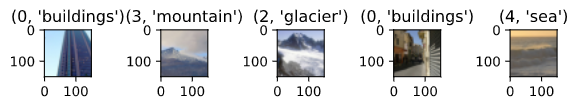
\includegraphics[scale=0.68]{assets/s6.png}
\end{center}

Five random images are chosen from images under \textit{src/data/predict/} directory. These images do not have label, so we are going to evaluate based on our knowledge whether the prediction is acceptable. The result is quite impressive as all five images are classified into their correct categories despite abut 82\% accuracy on testing data.

% ==========================================================================

\section{Performance and Discussion}

% ==========================================================================

\section{Conclusion}

% ==========================================================================

% \begin{thebibliography}
% % reference
%     \bibitem{Chollet_2017_CVPR}
%     % \bibitem{reference}
%     % \textbf{[1] }author name
%     % \textit{reference name}.
%     % publication
    
%     % \bibitem{reference1}
%     % \textbf{[1] }author name
%     % \textit{reference name}.
%     % publication

% \end{thebibliography}

\end{document}
